\let\counterwithout\relax
\let\counterwithin\relax
\documentclass[final]{fhnwreport}       %[mode] = draft or final
\usepackage{color, colortbl}
\usepackage{rotating, rotfloat,ragged2e, hyphenat, diagbox, wrapfig}
\definecolor{grau}{gray}{0.9}
\definecolor{hellgrau}{gray}{0.95}

                                        %{class} = fhnwreport, article, 
                                        %          report, book, beamer, standalone
\input{header}			                %loads all packages, definitions and settings												
\title{Kleinwasserkraftwerk}          	%Project Title
\author{Pflichtenheft}          		%Document Type => Technical Report, ...
\date{Windisch, 22.11.2018}             %Place and Date

\begin{document}

%%---TITLEPAGE---------------------------------------------------------------------------
\selectlanguage{ngerman}                %ngerman or english
\maketitle

\vspace*{-1cm}						    %compensates the space after the date line.
\vfill
\begin{figure} [H]
	\centering
	\includegraphics[width=11cm]{parkAvenue.jpg}
	\label{fig:Park_Avenue_432}
\end{figure}
\vfill

{
\renewcommand\arraystretch{2}
\begin{center}
\begin{tabular}{ >{\bf} l p{10cm} l }
Hochschule&Hochschule für Technik - FHNW\\
Studiengang&Elektro- und Informationstechnik\\
Autoren&Gruppe 4\\%Bachmann Lars \newline  Fischer Roni \newline Imhof Frank \newline Puschmann Pascal\\ 
Betreuer&Pascal Buchschacher \newline Anita Gertiser\\
Auftraggeber&Felix Jenni\\
Version&1.0 %Normally not used!
\end{tabular}
\end{center}
}

\clearpage

%\selectlanguage{ngerman}				%ngerman or english
\thispagestyle{empty}
			
%%---TABLE OF CONTENTS-------------------------------------------------------------------
\pagenumbering{Roman}		
%\selectlanguage{ngerman}				%ngerman or english
\tableofcontents
\clearpage

%%---TEXT--------------------------------------------------------------------------------
\pagenumbering{arabic}
\section{Übersicht} \label{sec:uebersicht}
\subsection{Ausgangslage}
Der Auftrag des Projekts 1 ist der Ersatz von Fossilen Ressourcen durch Elektrizität an einem ausgewählten Produkt. Das Team 4 hat sich das Ziel gesetzt, Lösungen zu finden, um die potentielle Energie des fallenden Abwassers in Hochhäusern und Wolkenkratzern in elektrische Energie umzuwandeln. Wird diese Energie zurück ins Gebäude gespeist, leistet unsere Lösung zwar keinen Ersatz von fossilen Ressourcen, aber einen Beitrag zur Reduktion des fossilen oder elektrischen Energieverbrauchs innerhalb von Gebäuden.
Durch die Recherchearbeit konnte das Team drei potentielle Lösungen finden, die nun in diesem technischen Teil des Pflichtenhefts weiter ausgearbeitet werden.

\subsection{Ziele}
Folgende Ziele hat sich das Team 4 in Absprache mit Herrn Jenni gesetzt:
\begin{table}[H]
\begin{tabular}{l}
1. Vorhandenes Potential mit Hilfe eines Modellhochhauses berechnen\\
2. Wirtschaftlichkeit der verschiedenen Lösungen untersuchen\\
\end{tabular}
\end{table}

\subsection{Nicht-Ziele}
Folgende Ziele wurden nicht verfolgt:
\begin{table}[H]
\begin{tabular}{l}
1. Respektierung der Normen\\
2. Absprache mit Architekten halten über Platzverhältnisse\\
3. Realisierung\\
4. Ausmasse der Bestandteile genau bestimmen\\
\end{tabular}
\end{table}
\subsection{Anforderungen}
Anforderungen an die potentielle Lösung sind die folgenden:\\
\begin{table}[H]
\begin{tabular}{lll}
Anforderung											&Mindest-Anforderung																		&Wunsch-Anforderung\\
\textbf{1. Technische Anforderungen}					&																						&\\
\qquad 1.1. Komplexität								&																						&\\
\qquad 1.2. Wirkungsgrad								&> 0.85																					&>0.9\\
\qquad 1.3. Stabilität								&																						&\\
\textbf{2. Finanzielle Anforderungen}				&																						&\\
\qquad 2.1. Amortisationszeit						&5 Jahre																					&3 Jahre\\
\textbf{3. Praktische Anforderungen}					&																						&\\
Wartungs	intervall									&>5 Jahre																				&10 Jahre\\          
\end{tabular}
\end{table}

\section{Lösungskonzept} \label{sec:loesungskonzept}
\subsection{Problemstellung} \label{subsec:problemstellung}
Um eine erste Übersicht der möglichen Probleme des Lösungskonzepts zu erhalten, wurden folgende Punkte im Brainstormingverfahren zusammengetragen:
\begin{figure}[H]
	\centering
	\includegraphics[width=1\linewidth]{Problemstellung_2.png}
	\caption{Baumdiagramm des Lösungskonzepts}
	\label{fig:Figure}
\end{figure}
\newpage

\subsection{Grobkonzept 1} \label{subsec:grobkonzept1}

\subsection{Grobkonzept 2} \label{subsec:grobkonzept2}
\begin{table}[H]
\small
\begin{tabular}{>{\HY\RaggedRight}p{3cm} >{\HY\RaggedRight}p{3.6cm} >{\HY\RaggedRight}p{6.9cm} r}
\hline
\textbf{Bestandteil}&\textbf{Typ}&\textbf{Funktion}&\textbf{Anz.}\\
\hline

\rowcolor{hellgrau}
\multicolumn{4}{l}{\textbf{Stromerzeugung}}\T\\
Turbine&Pelton&Umwandlung in Rotationsenergie&1\\
Generator&AC&Umwandlung in elektrische Energie&1\\
Wechselrichter&&Einspeisung ins Stromnetz&1\B\\

\rowcolor{hellgrau}
\multicolumn{4}{l}{\textbf{Kontrollsystem}}\T\\
PC&&Anlagesteuerung&1\\
SPS&Beckhof&Analoge und Digitale Aus- und Eingänge&1\B\\

\rowcolor{hellgrau}
\multicolumn{4}{l}{\textbf{Abwassertechnik}}\T\\
Tanks&&Zwischenspeicher für Abwasser&5\\
Ablassventil&&Entlässt das Abwasser aus dem Tank&5\\
Entlüftung&&Ermöglicht Luftaustausch, entlässt Gase&5\\
Notüberlauf&&Verhindert, dass Tank zu voll wird&5\\
Füllstandsensor&Vibronik Grenzschalter &Misst den Füllstand des Tanks&5\\
Druckleitungen&&Können Druck standhalten&5\\
Bypass für Turbine&&Ermöglicht Wartung der Turbine&1\\
Bypass für Tanks&&Ermöglicht Wartung \& Reingung der Tanks&5\\
Einwegventile&&Verhindern Rückfluss&4\B\\
\hline
\end{tabular}
\caption{Bestandteilliste Grobkonzept 2}\label{tab:BLGrobkonzept2}
\end{table}
Im Grobkonzept 2 soll die Energieausbeutung gesteigert werden, indem das Abwasser zuerst in Tanks gespeichert wird, die all 14 Stockwerke eingebaut sind. In unserem Hochmausmodell (Park Avenue 432) gibt es nach 12 Stockwerken jeweils zwei Zwischenstockwerke, wo der Einbau möglich wäre. Wenn der Füllstandsensor im Tank erkennt, dass er voll ist, wird das Ventil geöffnet und das Abwasser fliesst durch die Druckleitung in den Keller, wo es eine Pelton-Turbine mit Generator antreibt. Die gewonnene elektrische Energie wird über einen Wechselrichter dem Stromnetz zugeführt. \\ 
Das Abwasser füllt das Rohr komplett, so dass es keinen Luftwiderstand gibt, der es abbremst. So kann der Wirkungsgrad des Systems verbessert werden. Nur für eine Kurze Zeit, bis das Rohr komplett mit Wasser gefüllt ist, tritt Luftwiderstand auf.\\
Da es im Modellhochhaus in den letzten 17 Stockwerken kein Zwischenstockwerk mehr gibt, bleibt das Abwasser dieser Stockwerke ungenutzt.\\
Die baulichen Massnahmen, die nötig sind, um dieses System zu installieren sind beträchtlich. Es müssen Tanks eingebaut und Druckleitungen zur Turbine verlegt werden, welche im Keller installiert werden muss. Die bestehenden Abwasserleitungen müssen neu so verlegt werden, dass sie in die Tanks führen. Somit ist es eher für Neubauten geeignet als zur Nachrüstung.
\newpage

\begin{wrapfigure}{r}{0.5\textwidth}
  \begin{center}
    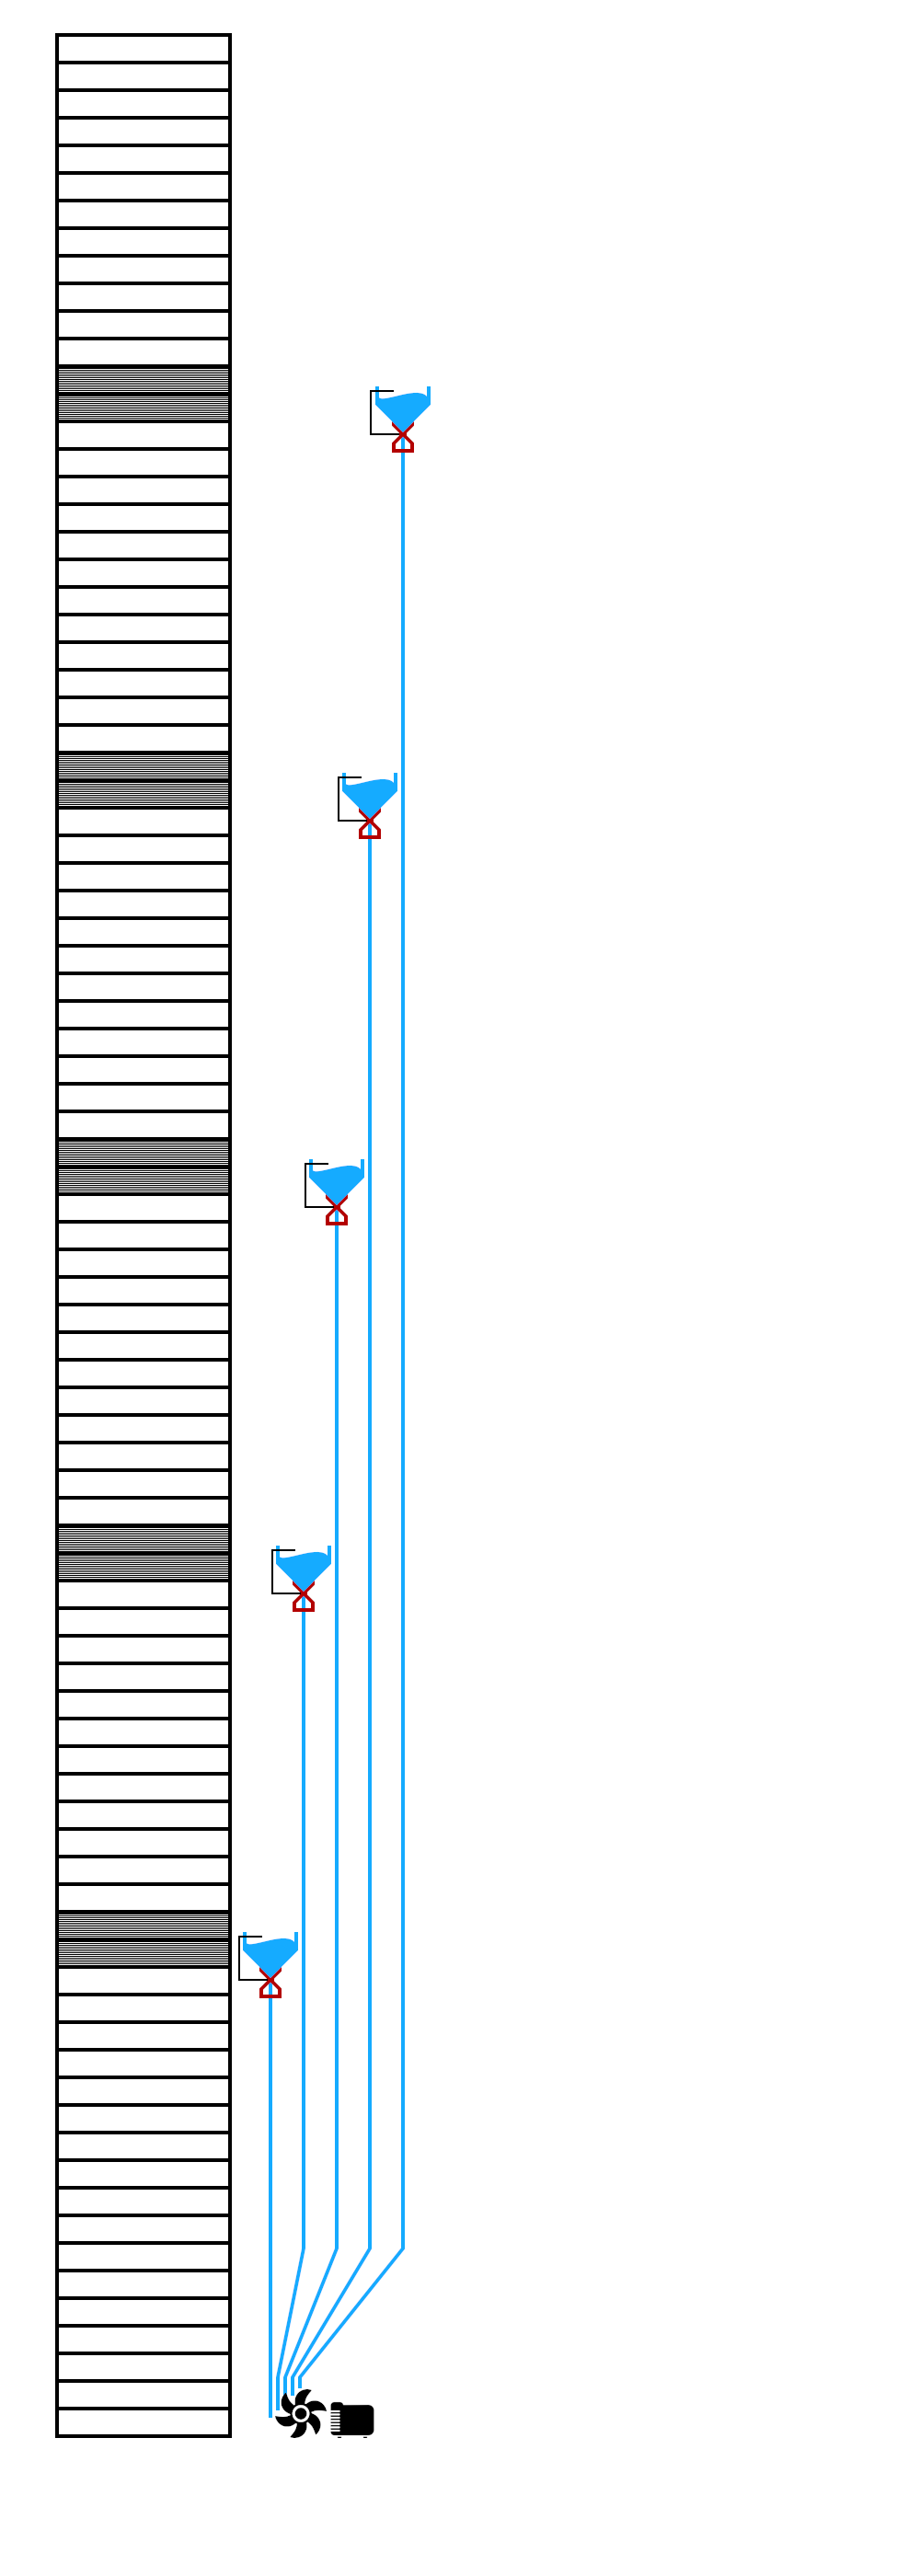
\includegraphics[width=0.48\textwidth]{grobkonzept2}
  \end{center}
  \caption{Schema Grobkonzept 2}
\end{wrapfigure}




Um zu verhindern, dass es in den Tanks zu Ablagerungen kommt, ist der Boden der Tanks trichterförmig. Ablagerungen werden dadurch beim Öffnen des Ventils weggespült. Sollte es trotzdem nötig sein, die Tanks zu reinigen, gibt es einen Bypass, mit dem das Abwasser am Tank vorbeigeführt werden kann.
Er kann dann entleert und gereinigt oder repariert werden. Auch die Turbine hat einen Bypass, der Wartungsarbeiten ermöglicht.

Jeder Tank ist mit einem Überlauf ausgestattet, der verhindert, dass ein Tank zu voll wird wenn z.B. der Ablauf verstopft ist. Das überschüssige Abwasser wird dann in einem Rohr in die Fallleitung wenige Stockwerke tiefer geleitet. Von dort gelangt es in den nächsten Abwassertank. Der Füllstandsensor im Tank erkennt, wenn der Pegel zu hoch wird und sendet eine Warnung.
Falls aus irgendeinem Grund mehr als eines der Ventile gleichzeitig geöffnet würde, könnte es zu einem Rückstau kommen, bei dem Abwasser durch die Druckleitungen vom höher gelegenen Tank in einen tieferen fliesst. Um dies zu verhindern, werden in den Druckleitungen Einwegventile eingebaut. Der höchstgelegene Tank benötigt kein solches Ventil. 

Ein Kontrollsystem steuert die Anlage und überwacht die Energiegewinnung und schreitet bei Störungen ein. Die Gewonnene Energie kann ins Netz zurück gespeist werden.

\bigskip

\textbf{Vorteile:} 									\newline
+	Luftwiderstand nur während Füllung				\newline
+	Nur eine Turbine									\newline
+	Keine AC-DC-AC Umwandlung						\newline
+	geregelte Wasserflussmenge						\newline

\textbf{Nachteile:}									\newline
-	braucht sehr viel Platz 							\newline
-	bauliche Massnahmen								\newline
-	Luftwiderstand während Füllung					\newline
- 	lange Druckleitungen								\newline
-	Abwasser der untersten 17 Stockwerke ungenutzt	\newline
\WFclear

\subsection{Grobkonzept 3} \label{subsec:grobkonzept3}

\begin{table}[H]
\begin{tabular}{>{\columncolor{hgelb}}l>{\columncolor{dgelb}}l>{\columncolor{hgelb}}llllll>{\columncolor{hgruen}}l>{\columncolor{dgruen}}l>{\columncolor{hgruen}}ll}
%GELBE KOLONNE						BLAUE UND PINKIGE KOLONNE										GRUENE KOLONNE
\titleCell{hgelb}{\textbf{Turbine}}	&&\titleCell{hblau}{\textbf{Elektrotechnik}}					&&\titleCell{hgruen}{\textbf{Abwassertechnik}}&\\
&\textbf{Turbinentyp}				&&&\cC{hblau}	&\cC{dblau}\textbf{Wechselrichter}	&\cC{hblau}	&&&\textbf{Tanks}				&&\\
&Pelton								&&&\cC{hblau}	&\cC{dblau}\textbf{Ventilsteuerung}	&\cC{hblau}	&&&Ablassentile					&&\\
&\textbf{Generatortyp}				&&&\cC{hblau}	&\cC{dblau}							&\cC{hblau}	&&&Entlüftung					&&\\
&Gleichstrom						&&&\titleCell{hblau}{ }											&&&Trichterförmig				&&\\
&\textbf{Anzahl}					&&&&&															&&&Füllstandssensor				&&\\
%ACHTUNG WEISSER ZWISCHENRAUM
&1									&&&\titleCell{hpink}{\textbf{Bedienung}}						&&&Notüberlauf					&&\\
&									&&&\cC{hpink}	&\cC{dpink}\textbf{Anzeige}			&\cC{hpink}	&&&\textbf{Druckleitungen}		&&\\
&									&&&\cC{hpink}	&\cC{dpink}der Füllstände			&\cC{hpink}	&&&Druckfestigkeit >40 bar		&&\\
&									&&&\cC{hpink}	&\cC{dpink}der Aktuellen Leistung	&\cC{hpink}	&&&\textbf{Bypass}				&&\\
&									&&&\cC{hpink}	&\cC{dpink}\textbf{Ventilsteuerung}	&\cC{hpink}	&&&für Tanks					&&\\
&									&&&\cC{hpink}	&\cC{dpink}							&\cC{hpink}	&&&für Turbine					&&\\
\titleCell{hgelb}{ }				&&\titleCell{hpink}{ }											&&\titleCell{hgruen}{ }&
\end{tabular}
\end{table}

Dieses Grobkonzept ist fast identisch zu Grobkonzept 2. Es gibt wieder einen oder mehrere Tanks, in denen das Abwasser zwischengespeichert wird. Allerdings gibt es nicht nur eine Turbine, sondern bei jedem Tank eine. Das Abwasser fliesst also immer von einem Tank in durch die Turbine in den darunterliegenden. Bei Grobkonzept 1 kann es relativ lange dauern, bis die Rohre komplett mit Wasser gefüllt sind. Bis das der Fall ist, kommt es zu Luftwiderstand in der Leitung. Bei jedem Tank eine Turbine einzubauen hat den Vorteil, dass die Rohre kürzer sind und so nach öffnen des Ventils schneller komplett mit Wasser gefüllt werden. So wird die Zeit verkürzt, in der Luftwiderstand auftritt. 

Vorteile 								\newline
+	Luftwiderstand tritt kürzer auf 	\newline
Nachteile	 							\newline
-	Braucht viel Platz					\newline
-	Grössere Bauliche Massnahmen nötig	\newline
-	Verstopfungsgefahr					\newline
-	Mehrere Turbinen nötig				


\subsection{Grobkonzept 4} \label{subsec:grobkonzept3}
\begin{table}[H]
\footnotesize
\begin{tabular}{>{\HY\RaggedRight}p{3cm} >{\HY\RaggedRight}p{2.2cm} >{\HY\RaggedRight}p{4cm} >{\HY\RaggedRight}p{3.3cm} >{\HY\RaggedRight}p{1.2cm}}
\hline
	\textbf{Bestandteil}		&\textbf{Typ}			&\textbf{Funktion}									&\textbf{Specs}			&\textbf{Anz.}\\
	\hline
\rowcolor{dgelb}
\multicolumn{5}{l}{\textbf{Stromerzeugung}}\\
	Wasserlift 				& 						&Umwandlung in Rotationsenergie						&							&5	\\
	Generator				&						&Umwandlung in elektrische Energie					&							&5	\\
\rowcolor{dblau}
\multicolumn{5}{l}{\textbf{Elektrotechnik}}\\
 	Wechselrichter			&						&Einspeisung ins Stromnetz							&							&1	\\
\rowcolor{dpink}
\multicolumn{5}{l}{\textbf{Bedienung}}\\
 	Anzeige 					&Display					&zeigt Tankfüllstände und Generatordaten an 			&							&1	\\
\rowcolor{dgruen}
\multicolumn{5}{l}{\textbf{Abwassertechnik}}\\
Bypass						&Absperrklappe			&Umleitung für Wartungsarbeiten am Wasserlift 		&							&6\\
Bypass 						&in Wirklichkeit			&sind es viel mehr als 6								&5*13+16=					&81\\
Leitung						&						&für Wartungsarbeiten 								&							&1\\
\hline
\end{tabular}
\end{table}
Im Grobkonzepts 4 wird die potenzielle Energie des Abwassers mit der Wasserlifttechnik ausgenutzt. Das Abwasser fliesst in eine Schaufel und wird in der Schaufel im Rohr nach unten transportiert. Somit erhält der Lift eine Bewegung nach unten und entleert am tiefsten Punkt das Abwasser. Die Leitung ist nie komplett mit Wasser gefüllt, daher kommt es zu einem Luftwiderstand in der Leitung, der das Abwasser abbremst.
\newpage
\begin{wrapfigure}{r}{0.5\textwidth}
  \begin{center}
    \includegraphics[width=0.48\textwidth]{grobkonzept4}
  \end{center}
  \caption{Grobkonzept 4}
\end{wrapfigure}
Die 5 oberen Lifte haben eine Länge von 66.08m, der unterste Lift 80.24m. Für Wartungsarbeiten existiert eine zusätzliche Leitung, die mittels Bypass angesteurt wird.

\textbf{Vorteile:}							\newline
+	kostengünstig							\newline
											\newline
\textbf{Nachteile:}\newline
-	defekt anfälliger						\newline
-	umbau									\newline
-	Verstopfungsresistent					\newline	
\WFclear			
\newpage








\section{Auswertung} \label{sec:auswertung}

\section{Modell}
Für die Berechnung der potentiellen Energie benützen wir das Modell Park Avenue 432, eines der höchsten reinen Wohnhochhäusern auf der Welt. Die stolze Höhe und der über das ganze Gebäude gleichbleibende quadratische Grundriss sind ideal für unsere Berechnungen. Für die Wassermengenberechnung stützen wir uns auf die Angaben des durchschnittlichen Wasserverbrauch in Amerika pro Person und Tag: 314 L. (Cheryl A. Dieter and Molly A. Mauphin. Public Supply and Domestic Water Use in the United States, 2015)
\begin{figure}[H]
\centering
\includegraphics[width=\linewidth]{parkAvenue.jpg}

\end{figure}
\begin{table}[H]
\begin{tabular}{ll}
Name:				& Park Avenue 432\\
Höhe: 				& 426m\\          
Etagen:				& 88\\
Etagenhöhe:			&4.72m\\
Hoechste Etage:		&392.1m\\
Wohnungen:			&104\\
Speziell:			&alle 12 Etagen 2 Etagen leer\\           
\end{tabular}
\end{table}


\subsection{Energieberechnung} \label{subsec:energieberechnung}

Die Endgeschwindigkeit des Wassers kann mit folgender Formel berechnet werden:
\begin{center}
\(v = \sqrt{2 \cdot g \cdot h} \)
\end{center}

Die Einheit der Geschwindigkeit \(v\) ist \si{m/s}, das Schwerefeld \(g\) auf der Erde besitzt den Wert 9.81~\si{N/kg}, und die Höhe \(h\) hat die Einheit \si{m}.

\bigskip

Die Energie, die gewonnen werden kann, wird mit folgender Formel berrechnet:

\begin{center}
\(E =\frac 12\ \cdot m \cdot v^2\)
\end{center}

Die Energie \(E\) hat die Einheit \si{J}, die Einheit der Geschwindigkeit \(v\) ist \si{m/s}, und die Masse \(m\) hat die Einheit \si{kg}

\bigskip

Um die Leistung zu erhalten, muss die Masse pro Zeit(1s) einberechnet werden. Die Masse wird mit der Dichte und dem Volumenstrom ersetzt.

\begin{center}
\(P =\frac 12\ \cdot \varphi \cdot Q \cdot v^2\)
\end{center}

Die Leistung \(P\) hat die Einheit \si{W}, der Volumentstrom \(Q\) die Einheit \si{m^3/s}, die Dichte \(\varphi\) \si{kg/m^3} und die Geschwindigkeit \(v\) \si{m/s}.

\newpage

Mit diesen Mathematischen Grundlagen kann nun die Energie an unserem Modellhochhaus für beide Grobkonzepte berechnet werden. Für die Berchnungen wird angenommen das pro Wohnung 2.5 Personen leben und sie einen Durchschnittverbrauch pro Tag von 314\si{L} haben.

Bei 146 Wohnungen und 74 Nutzbaren Etagen leben 5 Personen pro Etage. Es wird somit 1570\si{L} pro Etage pro Tag verbraucht.

\bigskip

\paragraph{Grobkonzept 1} 



\paragraph{Grobkonzept 2}

Mit dem Grobkonzept 1 kommt man total auf ********. Mit dem Grobkonzept 2 kommt man total auf *******. Die Berechnungen sind im Anhang unter  ersichtlich \ref{subsec:grobkonzept1} \nameref{subsec:grobkonzept1} und \ref{subsec:grobkonzept2} \nameref{subsec:grobkonzept2} ersichtlich




\subsection{Kostenberechnung} \label{subsec:kostenberechnung}
\section{Detailkonzept} \label{sec:detailkonzept}

Das Konzept mit den Wasserliften ist am besten geeignet für unsere Anwendung. Es existieren bereits solche «Rohrkettenförderer», die jedoch Produkte hinaufbefördern. Wir nutzen dieses System um das Wasser nach unten zu befördern und dabei Energie zu gewinnen. Es werden insgesamt sechs Lifte benötigt. Fünf Lifte überwinden je 60.08\si{m} und der unterste Lift überwindet 80.24\si{m}. In der Abbildung \ref{fig:PrinzipGrobkonzept4} \nameref{fig:PrinzipGrobkonzept4} ist dies grafisch dargestellt.

\subsection{Elektronik}

\begin{figure}[H]
\centering
\includegraphics[width=\linewidth]{Skizze_GK4.png}
\caption{Prinzipschema}
\label{fig:Prinzipschema}
\end{figure}

\paragraph{Funktionsbeschreibung}

Die potentielle Energie des Abwassers wird über ein Laufrad in kinetische Energie umgewandelt. Mit einem Getriebe wird die vom Laufrad kommende Drehzahl dem Generator angepasst, dieser wandelt die kinetische Energie in elektrische um. Der Gleichrichter transformiert den 3 Phasen Drehstrom in einen 2 poligen Gleichstrom. Anschliessend wird durch ein DC-DC Konverter eine Rückkoppelung auf den Genreator verhindert. Weiter stellt der Konverter sicher, dass eine stabile Ausgangsspannung anliegt und das der DC-Bus galvanisch vom Generator und Wechselrichter getrennt ist. Die summierte Energie aller sechs Generatorenstränge wird über einen Wechselrichter ins Stromnetz eingespeist. Zur Überwachung und auch zur Ansteuerung der Umlenkventile im Wartungsfall wird eine SPS verwendet.

\paragraph{Generator}

%TODO Lars: Tagesgangkurve beschreiben und dadurch mindestleitung Generator (3kW) begründen: (Tagesenergie 191.1MJ)

\begin{figure}[H]
\centering
\includegraphics[width=\linewidth]{tagesGangKurve.png}
\caption{Typische Tagesgangkurve. \cite{peakWaterDemand}}
\label{fig:tagesGangKurve}
\end{figure}

%TODO Lars: Ausgesuchter Generator mit Kosten auflisten; Warum dieser Generator? Drehzahl beachten -> Zahnradsystem

\paragraph{Wechselrichter nach Generator}

%TODO Lars: Ausgesuchter Wechselrichter mit Kosten auflisten; Warum dieser Wechselrichter?

\paragraph{DC-DC Wandler}

%TODO Lars: Ausgesuchter DC-DC Wandler mit Kosten auflisten; Warum dieser DC-DC Wandler(Kein Strom darf zurückfliessen!)?

\paragraph{Wechselrichter für Netzeinspeisung} \label{par:WechselrichterNetz}

Damit die gewonnen Leistung in das Netz eingespiesen werden kann, muss der Wechselrichter folgende Eigenschaften aufweisen. 

\textbf{Leistung:}		9KW \newline
\textbf{Ausgang:}		3Phasen \newline
\textbf{Kosten:}		Die Kosten sollen möglichst gering gehalten werden. \newline

In der Förderungsanlage wird ein Asynchrongenerator verbaut. Die Firma Voltacon ist bekannt für ihre Hochleistungswechselrichter.

Das Model Hybrid Wechselrichter HSI10000 entspricht den gewünschten Anforderungen für unsere Förderungsanlage. Der Wechselrichter transformiert die 48VDC auf 230VAC mit einer Frequenz von 50\si{\hertz}. Das Gerät kann bis zu einer Leistung von 10KW erbringen. Mittels integrierten Displays kann die erbrachte Leistung zusätzlich abgelesen werden. 

Gemäss Datenblatt lassen sich Ströme bis 200A regeln. Der Wechselrichter hat einen netzunabhängigen Energiespeicher (Batterie-Backup). Um die Daten des Wechselrichters weiterzuleiten stehen verschieden Kommunikationsmittel zur verfügung. Die Informationen können über einen USB Port, RS-232 oder den SNMP (Simple Network Management Protocol) Überwachungssoftware für Echtzeitstatusanzeige und-steuerung übermittelt werden. Die kosten des Wechselrichters belaufen sich auf 3'401\si{Fr}.


\paragraph{Kontrollsystem}

Das Kontrollsystem steuert und überwacht die Anlage und ist wie folgt aufgebaut: Auf einem PC ist eine C\# Software installiert. Das Programm kommuniziert über ModbusTPC mit der SPS und kann die Anlage so steuern. Über eine GUI kann ein Benutzer einfach auf die Anlage zugreifen, steuern und Informationen ablesen. Das Programm hat zwei verschiedene Modi. Einen Manuellen-Modus und einen Betriebs-Modus. Im Manuellen-Modus kann der Betrieb der Anlage für Wartungsarbeiten angepasst werden. So können die Ventile einzeln oder blockweise geschaltet werden. Im Betriebs-Modus werden nur im Störungsfall die Ventile automatisch geschalten um die Sicherheit zu gewährleisten. Wenn möglich werden nur einzelne Blöcke deaktiviert damit die Anlage weiterhin Strom produzieren kann. In beiden Modi wird die Stromgewinnung überwacht. So wird angezeigt welcher Generator gerade Strom erzeugt. Der Wechselrichter, der unter Wechselrichter für Netzeinspeisung beschrieben ist, kann über einem USB-Port eine serielle Kommunikation mit dem PC aufbauen. Das Programm kann die Informationen der aktuellen Energiegewinnung über diese Schnittstelle auslesen, speichert diese in einem Log. File und gibt diese an die Benutzeroberfläche weiter. Die gesammelten Daten können im Programm ausgewertet und grafisch dargestellt werden. Für dieses Kontrollsystem werden folgende Komponente benötigt.

\begin{table}[H]
\begin{tabular}{lllll}
\textbf{Anzahl}&\textbf {Komponente}&\textbf{Bezeichnung}&\textbf{Stückpreis [\si{Fr}]}&\textbf{Gesamtpreis [\si{Fr}]}\\
\hline
1&Kontrollklemme&BK9050&200&200\\
20&Digitale Ausgangsklemme&KL1114&100&2000\\
20&Digitale Eingangsklemme&KL2134&100&2000\\
7& Analoge Eingangsklemme&KL2134&100&700\\
1&PC&Dell&1000&1000\\
\hline
\end{tabular}
\end{table}

Die Kosten für die Komponenten betragen 5900 \si{Fr}. Für die Entwicklung der Software werden 3 PM benötigt und kostet einmalig 48'000\si{Fr}. 

\newpage


\subsection{Mechanik}

\paragraph{Rohrkette}

In der Industrie werden Rohrkettenförderer für den Transport von Schuttgüter verwendet. In der Abbildung \ref{fig:Rohrkettenfoerderer} \nameref{fig:Rohrkettenfoerderer} ist der Innenaufbau eines solchen Rohrkettenförderers ersichtlich.

\begin{figure} [H]
	\centering
	\includegraphics[width=6cm]{Rohrkettenfoerderer.jpg}
	\caption{Innenaufbau Rohrkettenförderer \cite{abconvey}}
	\label{fig:Rohrkettenfoerderer}
\end{figure}

Wir wollen keinen Schutt nach oben befördern, daher muss dieses System auf unsere Anforderungen angepasst werden. Diese Anforderungen sind, dass die verwendeten Materialien Robust gegenüber Korrasion sind, da das Abwasser aggressiv auf diese wirkt. Weiter müssen, um einen möglichst hohen Wirkungsgrad zu erreichen, die Platten mit möglichst kleinem Spielraum zur Ausserwand konstruiert werden, damit das Wasser nicht einfach auf der Seite herunterfliessen kann und gleichzeitig nicht eine zu grosse Reibung erzeugt wird. Die Drehachse, an dem der Generator angeschlossen wird ist ein Stösselkettenrad. Dieser ist in der Abbildung \ref{fig:stoesselkettenrad} \nameref{fig:stoesselkettenrad} zu sehen

\begin{figure} [H]
	\centering
	\includegraphics[width=6cm]{Stoesselkettenrad.jpg}
	\caption{Stösselkettenrad \cite{schrage}}
	\label{fig:stoesselkettenrad}
\end{figure}


Um diesen Wasserlift zu bauen beauftragen wir die Firma Schrage, ein führender Speziallist für Rohrketten, die in Deutschland zu Hause ist, beauftragt. Die Kosten belaufen sich für die 60.08\si{m} Höhendifferenz auf ca. 10'000\si{Fr} pro Lift und für die 80.24\si{m} Höhendifferenz auf ca. 13'000\si{Fr}. Insgesamt würde die Analage mit den Rohrketten, Rohr und Stösselkettenrad ca.63'000\si{Fr} kosten. \cite{schrage}

\newpage

\paragraph{Zahnradsytem}
%TODO Lars: Mindestdrehzahl dem Generator anpassen. Raddurchmesser für den Richtiungswechsel der rohrketten. Einen guten Wert annehmen

\paragraph{Umleitventil}

%TODO Roni: Ventile aussuchen die das Wasser entweder in die Falleitung oder in das rohrketten rohr leitet
% Genaues Ventil aussuchen. Anforderung 24V, Korrisionsbeständig

Da wir für Störungsfälle eine Fallleitung eingeplant haben, muss ein Umleitungsventil installiert werden. Das Model F7125 3-Way Butterfly Valve ist optimal für diese Bedingung geeignet. Das zugehörige Steuerungsmodel PRXUP-3-T kann von einer Spannung von zwischen 24V-230V angesteuert werden, somit können wir es im SPS System integrieren.

\textbf{Preis Bypass:  \si{Fr} \newline
 

\cite{F7125}
\subsection{Kosten}

%TODO Sonntag: Alle Kosten zusammentragen
\section{Wirtschaftlichkeit} \label{sec:wirtschaftlichkeit}
In diesem Abschnitt berechnen wir anhand grober Schätzungen die Wirtschaftlichkeit unseres Systems. 
Als Indikator für die Wirtschaftlichkeit wird die Amortisationszeit verwendet.
\subsection{Annahmen}
Für die vereinfachung der Amortisationsrechnung wurden folgende Annahmen getroffen:\\
\begin{itemize}  
\item Das Hochhaus wird neu gebaut, deshalb entstehen keine Umbaukosten.
\item Als Investitionskosten zählen wir die Einbaukosten der zusätzlichen Infrastruktur, die Materialkosten und die Entwicklungskosten.
\item Pro Jahr entsteht ein Serviceaufwand in der Höhe von schätzungsweise 3000 CHF.
\item Die Einbaukosten der zusätzlichen Infrastruktur betragen etwa 10000 CHF.
\end{itemize}

\subsection{Amortisationszeit}
Amortsierungszeit = Investitionskosten (Einbaukosten plus Materialkosten plus Entwicklungskosten) geteilt durch (jährlicher Rückfluss = (Stromgewinn minus Serviceaufwand)

\section{Projektvereinbarung} \label{sec:projektvereinbarung}
\begin{tabular}{l l}
\textbf{Auftraggeber} &\\
&\\
Jenni, Prof. Dr. Felix& \\
&\\
&\\
&\\
\rule{6cm}{0.5pt} & \rule{6cm}{0.5pt}\\
Ort, Datum & Unterschrift\\
&\\
&\\
&\\
&\\
&\\
&\\
\textbf{Projektleiter} &\\
&\\
Imhof, Frank &\\
&\\
&\\
&\\
\rule{6cm}{0.5pt} & \rule{6cm}{0.5pt}\\
Ort, Datum & Unterschrift\\
\end{tabular}



%%---BIBLIOGRAPHY------------------------------------------------------------------------

{\sloppypar
\selectlanguage{english}	
\setlength{\bibitemsep}{\baselineskip}
\printbibliography[heading=bibintoc]
\label{sec:lit}
}

%%---Anhang------------------------------------------------------------------------

\section{Anhang}

\subsection{Energieberechnung Grobkonzept 1}

\subsection{Energieberechnung Grobkonzept 1}


%%---NOTES for DEBUG---------------------------------------------------------------------
\ifdraft{%Do this only if mode=draft
%%requires \usepackage{todonotes})
\newpage
\listoftodos[\section{Todo-Notes}]
\clearpage
}
{%Do this only if mode=final
}
\end{document}
